\documentclass[a4paper,12pt]{article}

\usepackage{titlesec}
\titleformat{\paragraph}[runin]
{\normalfont\bfseries}{\thesubsection.\arabic{paragraph}}{1em}{}

% Réinitialiser le compteur de \paragraph pour qu'il soit associé à \subsubsection
\setcounter{paragraph}{0}

\usepackage{hyperref}
\usepackage[utf8]{inputenc}
\usepackage[T1]{fontenc}
\usepackage[french]{babel}
\usepackage{graphicx}
\usepackage{titling}

\usepackage{geometry}
\geometry{top=2cm, bottom=2cm, left=2.5cm, right=2.5cm}

\begin{document}
	\begin{titlepage}
		\centering
		{\Huge \textbf{Jeu Conception Logiciel}} \\[1.5cm]
		Olivier Cochard \\
		\today \\[2cm]
		
		
		
		
		{\Large Rapport de projet} \\[0.5cm]
		{\large \textit{Université de Caen Normandie}} \\[2cm]
		\includegraphics[width=0.3\textwidth]{Logo_Université_de_Caen_Normandie_2018}
		
		
		
		\vfill
		{\small Ce rapport a été rédigé dans le cadre du projet de Conception Logiciel, encadré par LETELLIER Guillaume.}
	\end{titlepage}
	
	\newpage
	\tableofcontents
	
	\section{Introduction}
	Ce rapport présente la conception et la réalisation d’un jeu de stratégie au tour par tour dans le cadre du devoir de Contrôle Continu de Génie Logiciel pour la licence 3 à l’Université de Caen. Ce jeu a été réalisé en monôme. L’objectif principal est de développer une application \textbf{robuste},\textbf{modulaire} et \textbf{extensible}, tout en respectant les bonnes pratiques enseignées au cours du semestre.
	
	Le jeu consiste en une simulation où au moins deux combattants s’affrontent sur une grille paramétrable en 2 dimensions, avec des règles précises concernant leurs mouvements, interactions et gestion de ressources. Le projet met particulièrement l’accent sur l’implémentation de patterns de conception (tels que \textbf{Proxy}, \textbf{Strategy}, et \textbf{Factory}) pour résoudre des problèmes spécifiques liés à la visibilité partielle du modèle et à la gestion des stratégies des joueurs.
	
	L'architecture est une séparation entre modèle, vue, contrôleur. Cette approche permet d'assurer une indépendance totale entre le contrôleur et la vue, laissant la possibilité d'y ajouter de futures extensions, comme par exemple une possibilité d'y jouer en réseau.
	
	Ce rapport va détailler les choix de conceptions, les algorithmes non triviaux, les soucis rencontrés, les améliorations apportées ou encore les parties qui auraient pu être approfondi.
	\newpage
	
	\section{Spécifications et Conception}
	\subsection{Diagramme des cas d'utilisation}
	Le principe de l'Observeur et l'Observable ici, permet de gérer la communication entre PlateauJeu et toutes les entités de ma grille. Après avoir reçut les information, mon Observeur se met à jour en conséquence et agis ensuite sur les Observables concernés.
	\begin{figure}[h!]
		\centering
		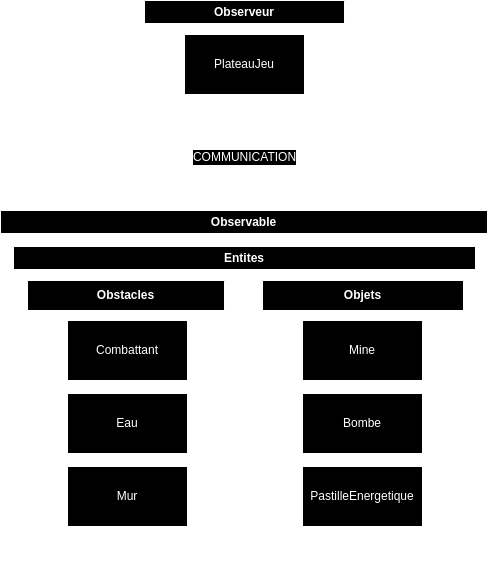
\includegraphics[width=0.3\linewidth]{diag_1}
		\caption{Diagramme de cas Observeur et Observable}
	\end{figure}
	
	A chaque changement de joueur courant une actions est attendu de ce combattant, si le combattant est un bot alors les actions seront définis par sa stratégie, tandis qu'un combattant contrôlé par l'utilisateur sera définis par les inputs du contrôleur.
	\begin{figure}[h!]
		\centering
		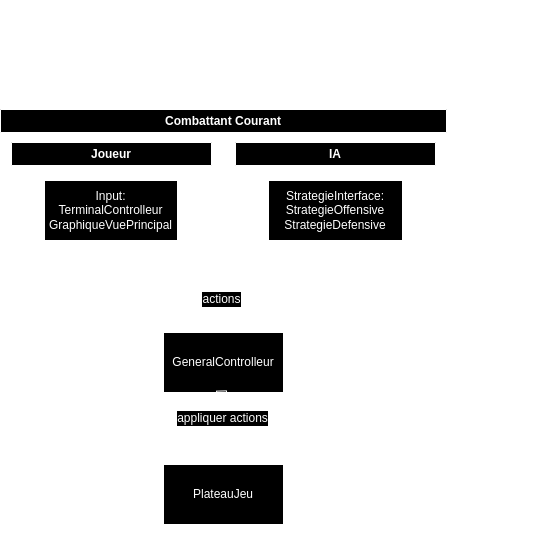
\includegraphics[width=0.3\linewidth]{diag_2}
		\caption{Diagramme de cas d'un tour du joueur courant}
	\end{figure}
	
	\subsection{Spécifications principales}
	Chaque combattant dispose d’une énergie, de munitions, d'une portée et de dégâts initiales. 
	L'énergie des combattants peut être affectée par les tirs, explosions, actions effectués et par les pastilles énergétiques.
	
	Les combattants peuvent se déplacer dans les quatre directions (haut, bas, gauche et droite).
	Une carte de jeu possède deux grille, la première contient tous les obstacles (mur, eau et combattant) qui ne sont pas traversable par les déplacements, et la deuxième ne possède que des objets (mine, bombe, et pastilles énergétiques) qui sont eux traversables par les combattants.
	
	Les actions disponibles sont les suivantes, on peut poser des pièges (mine, bombes), tirer (verticalement, horizontalement), utiliser un bouclier, se déplacer ou passer son tour.
	
	Les pièges explosent dès qu'un joueur marche dessus, les bombes explosent après un délai t (en nombre de tour), et les mines ne sont visibles que par le combattant poseur. Les explosions impactent les 9 case voisines et en cas de combattants leur réduisent leurs énergie.
	
	Lorsqu'un combattant n'a plus d’énergie alors celui-ci disparaît de la carte, la partie se termine si le nombre de survivants est inférieur ou égale à 1.
	
	Les vues (graphique et terminal) montrent un mélange des deux grilles, chaque joueurs voit une version unique différentes de la grille en fonctions des mines qu'ils ont posé. Le jeu est jouable entre 2 et n joueurs et l'utilisateur peut contrôler entre 0 et n joueurs. 
	
	La carte est configurable plusieurs lois au choix peuvent influencer sa génération, elle fait la taille x*y, de nombreuses variables sont paramétrables dans le fichier: "dist/gameSettings.properties".
	
	Les bots régissent à des stratégies implémentées ce qui permet de tester différentes approches et de déterminer la meilleure stratégie pour les combattants.
	
	\section{Algorithme, stratégies et factories}
	
	\subsection{Algorithme}
	\subsubsection{PathFinding a*}
	\label{sec:PathFinding}
	Cet algorithme permet de chercher le meilleur chemin de coordonnées entre deux positions.Il permet par exemple de vérifier qu'une carte à sa génération ait tous ses points d'apparitions accessibles. Ou encore de trouver le chemin le plus optimisé afin d'atteindre un objectif (adversaire ou une pastille énergétique).
	
	L’algorithme pour fonctionner a besoin de deux grilles (obstacles, objets), deux coordonnées (départ, arrivée) et un combattant qui l'utilise.
	Le combattant permet de verifier s'il est au courant de l’existence de certaines mines possiblement invisibles afin de les esquiver.
	Il possède deux listes, une avec les coordonnées (noeuds) testé et un autre avec les coordonnées à tester rangée dans l'ordre croissant des plus rapides vers l'objectif.
	Dans la boucle qui cherche le chemin, le noeud avec le coût total le plus bas (coutG + coutH) est extrait de la liste ouverte, ensuite si le noeud courant est la destination, l'algorithme a trouvé un chemin. Il reconstruit le chemin en remontant les nœuds parents et le retourne et s'il n'est pas arrivé à destination, alors l'algo explore les voisins de noeud courant et chaque voisin est recalculé.
	
	Dans le pire des cas l'algo teste toutes les coordonnées, O(m * n * log(m * n)) où m et n sont les dimensions de la grille.
	En cas de réussite l'algo renvoie le chemin à l'envers.
	
	\subsection{Stratégies}
	\subsubsection{Carte génération}
	Cette interface de stratégie permet de générer une carte sous certaines règles, on peut y choisir la taille et le nombre de combattants.
	La stratégie impacte la génération au niveau du taux de murs, d'eau et de pastilles. Elle permet aussi de définir une distance minimale entre chaque points d'apparitions.
	\paragraph{Equilibré}
	La stratégie équilibré a les règles suivantes, 20/100 de murs, 10/100 d'eau et 5/100 de pastilles énergétiques. La distance minimale est la taille de la carte divisé par deux.
	\paragraph{Chaos}
	Cette deuxième stratégie ne possède pas de distance minimales entre les points d'apparitions. Et pour finit elle contient 40/100 de murs, 20/100 d'eau et 1/100 de pastilles.
	
	\subsubsection{Intelligence ordinateur}
	Cette dernière interface de stratégie permet de faire des choix d'actions à partir de priorités et du positionnement des autre Obstacle et Objets.
	En cas de placement de piège celui-ci est positionné de façon intelligente en étant la plus proche possible de l'adversaire. 
	\paragraph{Offensive}
	\label{sec:Offensive}
	Dans un premier temps la stratégie regarde si un tir vertical ou horizontale est intéressant.
	En cas d’égalité entre les deux directions, celle-ci est tiré aléatoirement. Si au moins un des deux est intéressant il y a 4 cas de figures:
	\begin{enumerate}
		\item Tir disponible => effectue un tir
		\item Tir indisponible (delaiTir > 0 ou munition <= 0) et bouclier disponible => se protège
		\item Tir indisponible, bouclier indisponible (délaiBouclier > 0) et distance avec la cible < 3 => place un piège
		\item Tir indisponible, bouclier indisponible et distance avec la cible > 2 => passer le tour
	\end{enumerate}
	Si un aucun tirs n'est intéressant, l'ia cherche l'entité la plus proche (pastille, adversaire), et avec l'algorithme PathFinfing cherche un chemin possible, il y a ici deux possiblités:
	\begin{enumerate}
		\item chemin existant => se rapproche de l'entité
		\item chemin null => passe son tour
	\end{enumerate}
	
	\paragraph{Défensive}
	\label{sec:Défensive}
	Cette classe regarde s'il existe une entité proche, s'il n'en existe pas le combattant passe son tour. Dans le cas normal ou il en existe une, l'ia regarde si elle possède un tir intéressant, et il y a  situations:
	\begin{enumerate}
		\item tir disponible => tirer sur adversaire
		\item distance adversaire < 6 => fuite à la case la plus éloigné de l'adversaire
		\item distance adversaire > 5 => placer des pièges ou passer son tour 
	\end{enumerate}
	
	\subsection{Factories}
	\paragraph{Combattant}
	\label{sec:stats}
	La classe CombattantFactory permet la génération de différents types de combattants parmi les suivants:
	\begin{enumerate}
		\item Classique
		\begin{enumerate}
			\item Énergie: 125
			\item Portée: 3
			\item Munition: 10
			\item Dégât: 25
		\end{enumerate}
		\item Sniper
		\begin{enumerate}
			\item Énergie: 100
			\item Portée: 5
			\item Munition: 10
			\item Dégât: 15
		\end{enumerate}
		\item Tank
		\begin{enumerate}
			\item Énergie: 150
			\item Portée: 1
			\item Munition: 10
			\item Dégât: 35
		\end{enumerate} 
	\end{enumerate}
	Elle permet aussi la génération d'un combattant aléatoire parmi ces trois différents types. 
	
	\paragraph{Carte}
	\label{sec:carte}
	En plus de la génération aléatoire j'y ai implémenté des cartes déjà générés en fonction du nombre de combattants demandés. Il existe quatre cartes avec les capacités suivantes: 2, 4, 6, 8 places.  
	\begin{figure}[h!]
		\centering
		
\includegraphics[width=1\linewidth]{legende}
		\caption{Légende elements interface graphique}
	\end{figure}
	\begin{figure}[h!]
		\centering
		\begin{minipage}{0.5\linewidth}
			\centering
			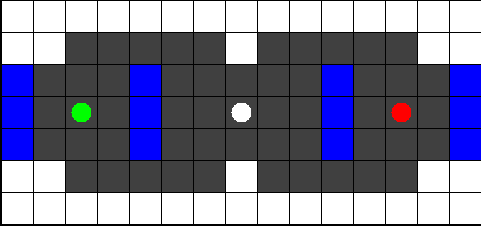
\includegraphics[width=\linewidth]{carte_1}
			\caption{Carte pour deux combattants}
		\end{minipage}\hfill
		\begin{minipage}{0.4\linewidth}
			\centering
			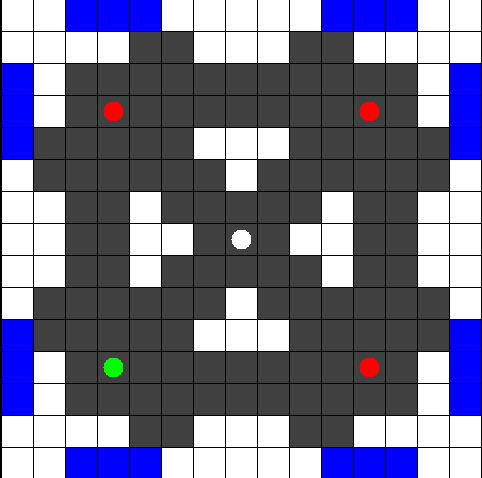
\includegraphics[width=\linewidth]{carte_2}
			\caption{Carte pour quatre combattants}
		\end{minipage}
		\vskip 10pt
		\begin{minipage}{0.3\linewidth}
			\centering
			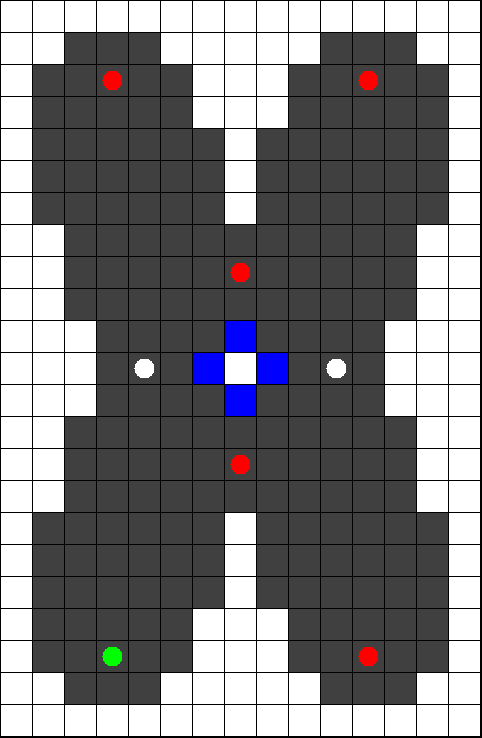
\includegraphics[width=\linewidth]{carte_3}
			\caption{Carte pour six combattants}
		\end{minipage}\hfill
		\begin{minipage}{0.4\linewidth}
			\centering
			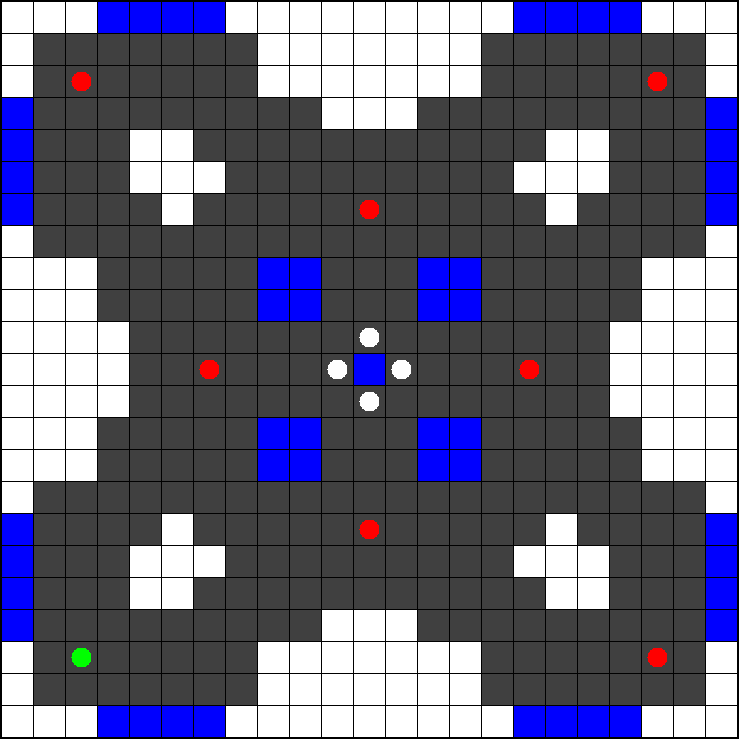
\includegraphics[width=\linewidth]{carte_4}
			\caption{Carte pour huit combattants}
		\end{minipage}
	\end{figure}
	
	\section{Amélioration effectués}
	\subsection{Map factory}
	Classe déjà expliqué plus haut ! 
	\hyperref[sec:carte]{-ici-}
	\subsection{Délai d'action}
	Ajout des variables delaiTir et delaiBouclier, je l'ai implémenté afin d'obtenir des stratégies d'ordinateurs plus intéressantes, ces délais permettent d’éviter le fait qu'un combattant puisse spammer une seule action en boucle. Cette implémentation permet plus de stratégies, d'anticipations et de combinaisons possibles. 
	\subsection{Statistiques unique pour chaque type de combattants}
	Cette implémentation avait pour but de diversifier les types de combattants. Les statistiques affectés sont la quantité d’énergie, la portée et les dégâts lors de tirs. La portée et les dégâts permettent d'établir des stratagèmes en conséquences. La diversité de portée permet aussi des interactions plus diversifiées entre les ordinateurs.
	\hyperref[sec:stats]{-ici-}
	\subsection{Eau}
	Je trouvais que mes cartes manquaient de diversité. Actuellement les murs bloquent les projectiles et bloquent les déplacements de joueurs. Je me disais qu'un élément bloquant les déplacements mais pas les tirs serait intéressant en plus d'améliorer le coté esthétique. 
	\subsection{Fichier de paramétrage}
	Il est embêtant de devoir recompiler à chaque modifications de variables, c'est pour quoi il était intéressant de répertorier de nombreux paramètres dans un fichier unique et de faire en sorte que ces variables dépendent d'un tout autre fichier modifiable tout le temps (sans recompilation).
	\subsection{Intelligence artificielle}
	Dans mon projet je trouvais que la deuxième stratégie était trop peu intéressante par rapport à la première, c'est pourquoi tous les ordinateurs dans le projet sont offensifs. 
	\paragraph{Offensive}
	Cette stratégie est assez développé et fonctionnelle. L'utilisation du PathFinding est très intéressante et puissante.  
	\hyperref[sec:Offensive]{-ici-}
	\paragraph{Défensive}
	Cette seconde stratégie est moins efficace mais a le mérite d'exister. 
	\hyperref[sec:Défensive]{-ici-}
	\subsection{PathFinding}
	Classe déjà expliqué plus haut ! 
	\hyperref[sec:PathFinding]{-ici-}
	Cet algorithme est aussi utilisé pour vérifier qu'une carte est valide a condition qu'un joueur à l'apparition puisse atteindre tous les autres joueurs.
	\subsection{Super build.xml}
	Actuellement je possède un build.xml par package seulement il en fallait un pour gérer la doc, le dist donc je l'ai amélioré afin de gérer la compilation, les tests et l’exécution du jeu. Voici les commandes disponibles:
	\begin{enumerate}
		\item ant javadoc (compilation, javadoc)
		\item ant jar (compilation, copy.jar, .jar executable)
		\item ant runTests (jar + execute tous les tests)
		\item ant run (jar + execute le .jar executable)
	\end{enumerate}
	
	\section{Conclusion}
	
	Le projet avait pour objectif de développer un jeu de stratégie au tour par tour, dans lequel des combattants s'affrontent sur une grille, avec des interactions telles que des déplacements, des tirs et des placements de pièges. 
	
	Le jeu a été implémenté avec succès, avec une logique de combat fluide et une interface graphique simple mais fonctionnelle. La gestion des obstacles, des tirs, des mines et des bombes a été correctement mise en œuvre, et le code respecte bien l'architecture de type MVC.
	
	Cependant, la gestion des stratégies des combattants robotisés n'a pas été aussi raffinée que prévu, notamment en raison du manque de temps pour tester différentes stratégies complexes, et de temps à investir dans la stratégie défensive. De plus l'interface de joueurs n'a pas été correctement implémenté par faute de temps, actuellement il n'y a qu'une seule interface principale qui s'adapte au joueur courant.
	
	Une amélioration possible serait d'ajouter des fonctionnalités multijoueurs en ligne, ce qui permettrait à plusieurs joueurs de s'affronter dans des parties en réseau. Une meilleure gestion de l'intelligence artificielle des robots serait également bénéfique pour rendre les parties plus intéressantes. Et un système d'équipe serait lui aussi très intéressant encore plus avec l'aspect multijoueur.
	
	En conclusion, ce projet m'a permis d'appliquer des concepts de programmation orientée objet, ainsi que des techniques de conception logicielle telles que l'architecture MVC et les design patterns. Cela a été une excellente occasion d'améliorer mes compétences en programmation et de renforcer ma compréhension des principes du génie logiciel. Et le fait d'avoir travaillé seul m'a aussi permis de toucher à tout et donc d'appendre d’avantage sur tous les domaines et emmener le projet dans la direction que je souhaitais sans contraintes.
\end{document}